\documentclass[a4paper]{article}

%% Language and font encodings
\usepackage[english]{babel}
\usepackage[utf8x]{inputenc}
\usepackage[T1]{fontenc}
\usepackage{subfig}

%% Sets page size and margins
\usepackage[a4paper,top=3cm,bottom=2cm,left=3cm,right=3cm,marginparwidth=1.75cm]{geometry}

%% Useful packages
\usepackage{amsmath}
\usepackage{graphicx}
\usepackage{wrapfig}
\usepackage{float}
\graphicspath{ {./img/} }
\usepackage[colorinlistoftodos]{todonotes}
\usepackage[colorlinks=true, allcolors=blue]{hyperref}

\title{\vspace{-2.5cm}Estimation of Hurst Parameter of Mono-fractal signals\\ EE-678, Wavelets, Prof. V.M. Gadre}
\author{Agrim Gupta, Saurabh Pinjani, Asim Ukaye \\ PhD Supervisor: Shivam Bhardwaj, MTech Mentor: Harsh Solanki}

\begin{document}
\maketitle

\begin{abstract}
In the main course assignment, we explored self similar signals and how to estimate them using techniques in wavelet domain. A good starting point was PCA Eigenspectrum paper [1] by Li et al. The proposed method works good for the H parameter in range (0.5,1) and doesn't scale up with sample size as well. Our proposed algorithm using detail coefficients of DWT improves upon these shortcomings. In addition, we studied and implemented paper on "Bayesian Estimation of $\gamma$ for 1/f signals" and experimented with different wavelet basis for the same, which hadn't been attempted by the authors before
\end{abstract}

\section{Introduction}

\subsection{Fractals}
In mathematics, a self-similar object is exactly or approximately similar to a part of itself  i.e. the whole has the same shape as one or more of the parts. Self-similarity is a typical property of fractals.

\begin{figure}[h]
    \centering
    \subfloat[Triangular Fractals]{{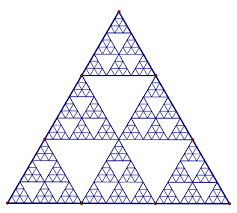
\includegraphics[width=5cm]{fractals_1.png} }}%
    \qquad
    \subfloat[Close-up of a Romanesco broccoli]{{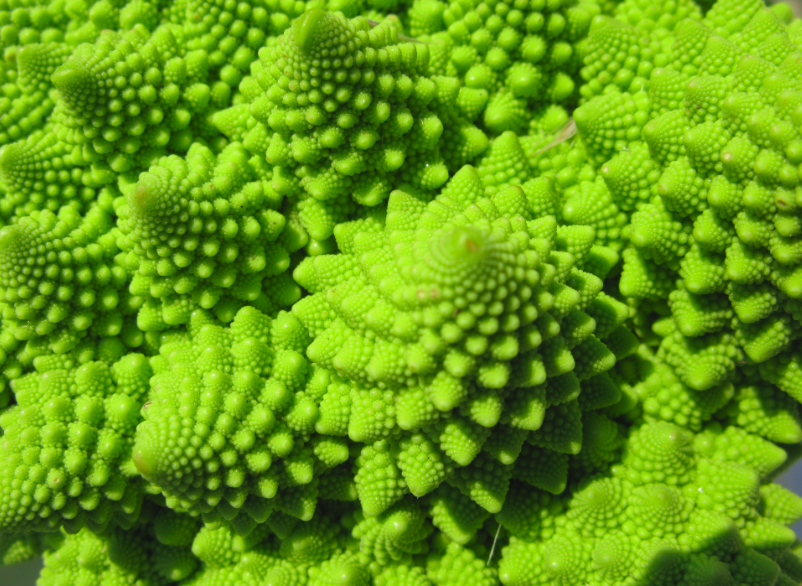
\includegraphics[width=5cm]{fractals_2.png} }}%
    \caption{Examples of fractals are abound.}%
    \label{fig:example}%
\end{figure}

\subsection{Self-Similar Signals}
A random process is said to be self-similar if its statistics are invariant to compressions and dilations of the waveform in time i.e. its statistical properties don’t change with scaling. In mathematical terms
$$x(t) \equiv a^{-H}x(at)$$
Here the ‘H’ in the exponent is called the Hurst Parameter. This parameter is used to characterize such self similar random processes. We will be looking at methods of extraction of this parameter going forward in this report.

\begin{figure}[h]
  \begin{minipage}[c]{0.67\textwidth}
    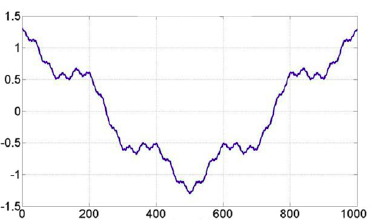
\includegraphics[width=\textwidth]{self_sim.png}
  \end{minipage}\hfill
  \begin{minipage}[c]{0.3\textwidth}
    \caption{
       Weierstrass signal is an example of a self-similar signal. If we cut out the part of the signal from t=400 to t=600, the part is similar to the whole.
    } 
  \end{minipage}
\end{figure}

In this report we will be primarily dealing with two particular classes of self similar signals :
(i) Fractional Brownian Motion  (ii) $\frac{1}{f}$ processes

\section{Self-similar Signals studied}
\subsection{Fractional Brownian Motion (fBm) signal}
fBm, a generalization of Brownian motion, is a continuous-time Gaussian process BH(t) on [0, T], which starts at zero, has expectation zero for all t in [0, T]​.
​Unlike classical Brownian motion, the increments of fBm need not be independent and can be positively or negatively correlated. The degree of correlation is what characterises the process and is captured in the Hurst parameter(H). When H assumes a value lower than 0.5 the increments are negatively correlated and for values above 0.5 they are positively correlated. If H is 0.5 the steps are uncorrelated and hence the fBm becomes a vanilla brownian motion.
It has the following covariance function [2].:
$$R_{B_H}(s,t)=E[B_H(s)B_H(t)]=\frac{V_H}{2}(|s|^{2H}+|t|^{2H}+|s-t|^{2H})$$
where $V_H=var[B_H(1)]=\frac{-\Gamma(2-2H)cos(\pi H)}{\pi H(2H-1)}$

We saw various forms of the covariance functions in [1],[2] and [3]. The most general version is presented above. 

\begin{figure}[h]
  \begin{minipage}[c]{0.6\textwidth}
    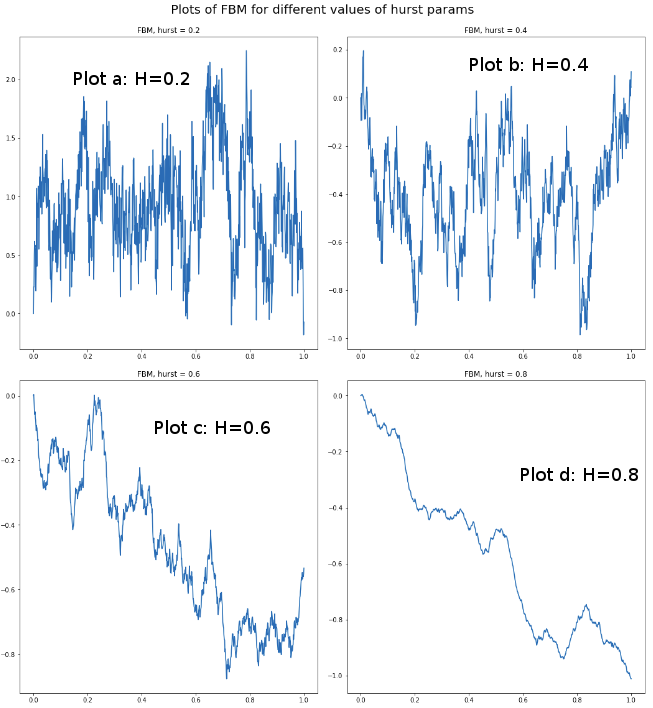
\includegraphics[width=\textwidth]{fbm_H2.png}
  \end{minipage}\hfill
  \begin{minipage}[c]{0.4\textwidth}
    \caption{
       The Hurst parameter fully characterizes a monofractal signal such as fBm. The graphs above
illustrate this point. In graph (a) H=0.2. Hence the incremental steps are negatively correlated
and hence the graph is tremulous. However in graph (d) where H=0.8 the graph is quite smooth
due to the positive correlation between subsequent steps. So therefore as we move from graph
(a) to (d) the graph gets smoother with an increasing Hurst parameter.
    } 
  \end{minipage}
\end{figure}

\subsection{1/f Processes}
This is a class of self similar signals that possess a power spectrum obeying the following law:
$$S(\omega)=\frac{\sigma_x^2}{|\omega|^\gamma}$$
where $\gamma=2H+1$. $\gamma$ typically lies between 0 and 2.
It is generally convenient to extend the notion of l/f processes to include nearly 1/f processes that are defined as having power spectra bounded according to:
$$\frac{k_1}{|\omega|^\gamma} \leq S(\omega) \leq \frac{k_2}{|\omega|^\gamma}$$
where $k_1$ and $k_2$ satisfy $0 < k_1 \leq k_2 < \infty $

\section{Extraction of Hurst Parameter in fBm}
Since the Hurst parameter characterises the fBm, its extraction from a given signal is a problem of great relevance. This has been studied in existing literature. The method discussed in literature is discussed below. We will also be analyzing its shortfalls and domain of applicability.

\subsection{H parameter estimation using PCA Spectrum (Li et al. 2009)}
\begin{wrapfigure}{r}{8cm}
\vspace{-15pt}
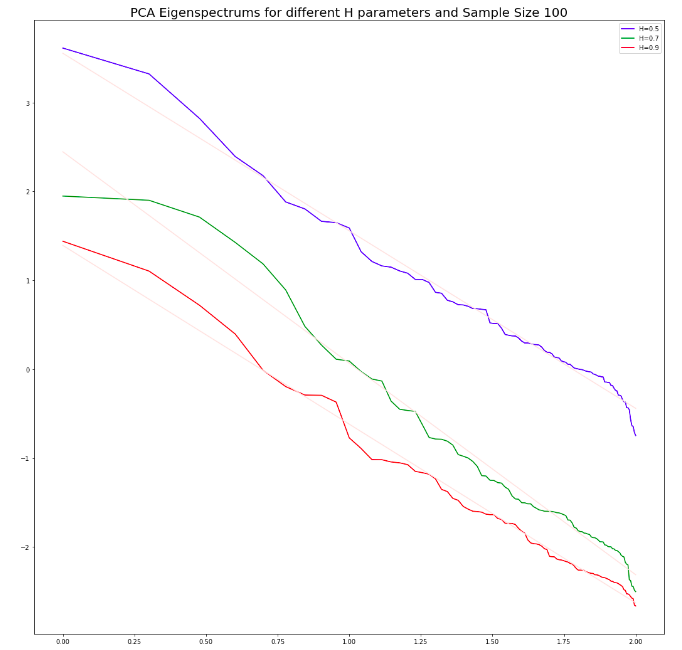
\includegraphics[width=8cm]{Li_1.png}
\end{wrapfigure} 
A method to estimate the hurst parameter from the PCA eigenspectrum of a FBM signal was proposed. The PCA eigenspectrum of the autocovariance matrix of FBM signal is linear in log log scale, and the slope is indicative of the Hurst parameter. The method was theoretically proved by showing equivalence of eigenvalues arising from discrete K-L expansion and autocovariance matrix. However this method is plagued with certain issues:
\begin{itemize}
\item This method works for signals with H in the range (0.5,1). This is a serious shortcoming as many signals in real life have negative correlation.
\item As sample size increased the difference between the estimated and actual value of Hurst increases. Ref. Figure below.
\end{itemize}
\begin{figure}[h]
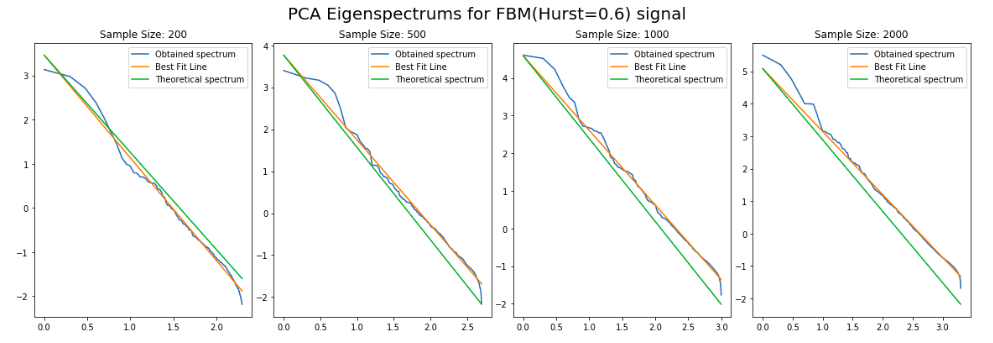
\includegraphics[width=\textwidth]{Li_2.png}
\caption{As Sample Size increases, deviation between actual slope and expected slope increases}
\end{figure}

\subsection{H parameter estimation using Eigenspectrum of Detail coefficients}
Instead of forming autocovariance matrix of the FBM signal, we first take DWT of the FBM signal. Then we use the detail coefficients (high pass branch) to form the autocovariance. Then we plot the eigenspectrum of the modified autocovariance matrix. However, instead of looking at the slope we look at the y-intercept. We can map the y-intercept (which is nothing but the highest eigenvalue) to the Hurst parameter.
Now to judge the effectiveness of the method we look at the graph for the PCA spectrum method reported in literature. One can clearly see that separability of the curves have increased in our method. Hence our method is clearly advantageous.

\begin{figure}[H]
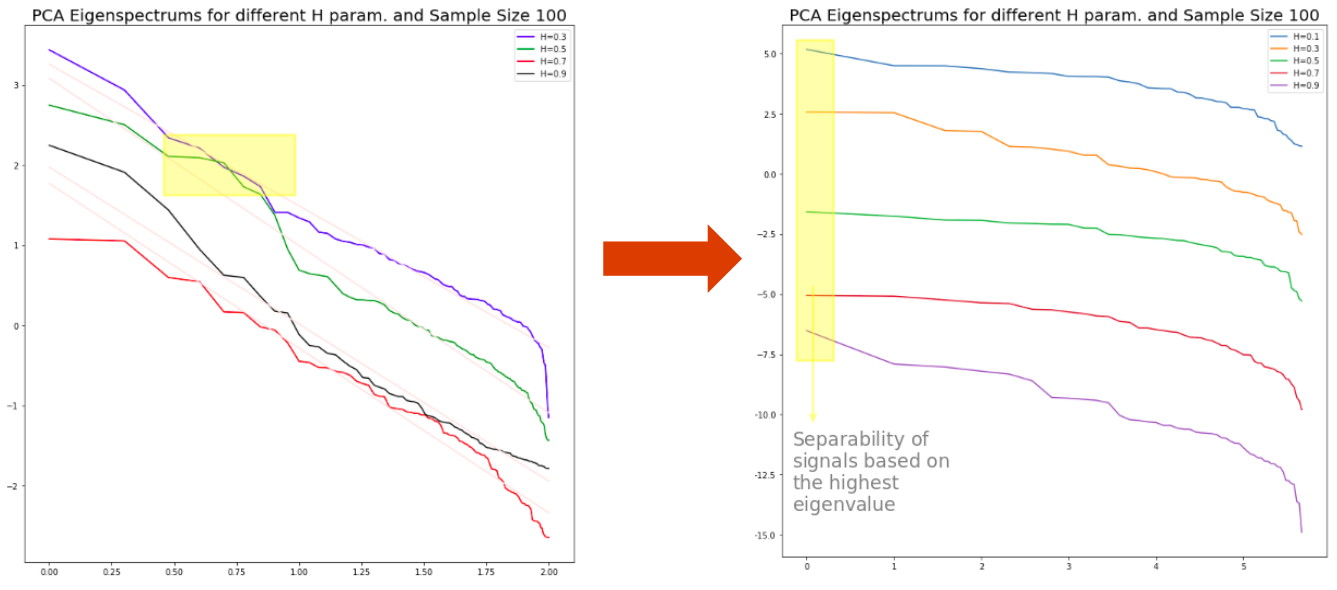
\includegraphics[width=\textwidth]{dwt_1.png}
\caption{Separability of curves generated by different H increases when eigenspectrum of detail coefficients is plotted}
\end{figure}

\begin{wrapfigure}{r}{7cm}
\vspace{-15pt}
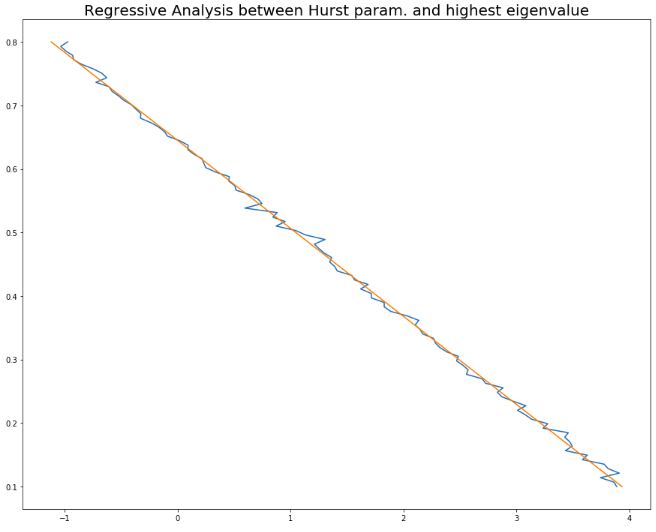
\includegraphics[width=7cm]{dwt_lin.png}
\vspace{-30pt}
\end{wrapfigure} 
Next step is to fit in the y highest eigenvalues against the Hurst parameter of the signal. A linear fit suffices and gives sufficiently good results, indicating the linear relationship between Hurst parameter and highest eigenvalue.  It is clear from the graph that this method gives a fairly accurate estimate of the Hurst parameter, even for hurst parameters in the range (0,0.5) which could not be obtained accurately via the PCA eigenspectrum method proposed by Li et al.
\\
\subsubsection{Mathematical analysis of the proposed method}
\subsubsection{Conclusion and Future Work Possible}
\section{Estimation of Fractality parameters (H \& $\gamma$) for \\1/f processes}
In our assignment we also aimed to study and implement [4] presented by Wornell and Oppenheim. This paper shows a robust, computationally efficient and consistent iterative algorithm to estimate Fractality Parameters (H), ​and variance estimates of 1/f processes using wavelet expansion
By implementing the ideas and algorithms proposed in this paper we were able to understand the wavelet domain analysis of fractals through implementation. We also aimed at replicating some of the results proposed in the paper and observe and comment on certain parts which the paper did not discuss, such as the effect of choice of wavelet basis on estimates of H.

The ultimate goal of this activity was to research the possibility of extending the framework (given for 1/f processes) of this paper to f-ARIMA processes.

\subsection{Outline of the paper}

\end{document}	